\chapter{Computing Response Functions \& Polaron Mobility}
\label{chap:fifth}

\thesisepisrcyear{What is the meaning of life?}{John Doe}{Thoughts}{1971}

\chapterintrobox{This is the introduction paragraph.}

\section{Polaron Mobility}
\label{sec:chap-fifth-first}

The polaron DC mobility may be obtained in the same way as was done for the Fr\"ohlich model from real components of the frequency- and temperature-dependent impedance function,

\begin{equation}\label{eqn:mobility}
    \mu_{dc} = \lim_{\Omega \to 0} \Re{\frac{1}{z(\Omega)}},
\end{equation}
where the impedance function is expressed in terms of the memory function $\Sigma(\Omega)$,
\begin{equation}
    z(\Omega) = i \left( \Omega - \Sigma(\Omega) \right).
\end{equation}
More specifically, we can express the inverse DC mobility just in terms of the memory function,
\begin{equation}
    \mu_{dc}^{-1} = \lim_{\Omega \to 0} \Im{\Sigma(\Omega)}.
\end{equation}
We start from an expression for the dynamical memory function for a general polaron and specialise in the Holstein case. The general memory function can be written as,
\begin{equation}
    \Sigma(\Omega) = \frac{4}{n m_b \hbar\Omega} \int_0^{\infty} dt\ \left(1 - e^{i \Omega t}\right) \Im \left\{ \sum_{\vb{q}} \abs{V_{\vb{q}}}^2 q^2 D_{\omega_{\vb{q}}}(t) \langle e^{i \vb{q} \cdot \left[ \vb{r}(t) - \vb{r}(0) \right]} \rangle \right\},
\end{equation}
where we assume the system to be rotationally invariant. Here $D_{\omega}(t)$ is the \emph{real}-time thermal and \emph{dynamical} phonon Green function,
\begin{equation}
    D_\omega(t) = \coth(\frac{\hbar \beta \omega}{2}) \cos(\omega t) - i \sin(\omega t),
\end{equation}
and can be obtained from substituting $\tau \to i t$ into Eqn.~(\ref{eqn:phonongf}).

The key term to evaluate is the density-density correlation function or dynamical structure factor,
\begin{equation}
    S_{\vb{q}}(t) = \langle \rho_{\vb{q}}(t) \rho^*_{\vb{q}}(0) \rangle = \langle e^{i \vb{q} \cdot \left[ \vb{r}(t) - \vb{r}(0) \right]} \rangle.
\end{equation}
As done earlier, the expectation value can be expressed as a path integral. However, even the full Fr\"ohlich model cannot be evaluated exactly. We approximate this by evaluating this expectation value with respect to the Feynman polaron model,
\begin{equation}
    \langle \rho_{\vb{q}}(t) \rho^*_{\vb{q}}(0) \rangle_0 = e^{-q^2 r_p^2 G(t)},
\end{equation}
where $G(t)$ is the polaron Green function evaluated in real-time (i.e. substitute $\tau \to it$ into Eqn.~(\ref{eqn:polarongreensfunc}),
\begin{equation}
    G(t) = i t \left(1 - \frac{i t}{\hbar \beta} \right) + \frac{v^2 - w^2}{v^3} \left[ D_v(0) - D_v(t)  - i v t \left(1 - \frac{i t}{\hbar \beta} \right) \right].
\end{equation}
In $n$-dimensions, we need to evaluate the reciprocal-space integral,
\begin{equation}
    \begin{aligned}
        I(n) &= V \int \frac{d^n q}{(2\pi)^n} \abs{V_{\vb{q}}}^2 q^2 D_{\omega_{\vb{q}}}(t) e^{-q^2 r_p^2 G(t)}, \\
        &= \frac{V \abs{S^{n-1}}}{(2\pi)^n} \int_0^R dq\ q^{n+1} \abs{V_{q}}^2 D_{\omega_{q}}(t) e^{-q^2 r_p^2 G(t)} ,
    \end{aligned}
\end{equation}
where we have used that the system is rotation-invariant. For a general polaron model, we then have the memory function,
\begin{equation}
    \Sigma(\Omega) = \frac{4}{n m_b\hbar\Omega} \frac{V \abs{S^{n-1}}}{(2\pi)^n} \int_0^\infty dt\ \left(1 - e^{i \Omega t}\right) \int_0^\Lambda dq\ \abs{V_{q}}^2 q^{n+1} \Im{D_{\omega_q}(t) e^{-q^2 r_p^2 G(t)}}.
\end{equation}
In the zero frequency limit, we have,
\begin{equation}
    \lim_{\Omega \to 0} \frac{\left(1 - e^{i \Omega t}\right)}{\Omega} \to -i t,
\end{equation}
so for the general polaron DC mobility, we get,
\begin{equation}
    \mu_{dc}^{-1} = -\frac{4 e^2}{n m_b \hbar} \frac{V \abs{S^{n-1}}}{(2\pi)^n} \int_0^\infty dt\ t \int_0^\Lambda dq\ q^{n+1} \abs{V_{q}}^2 \Im{ D_{\omega_{q}}(t) e^{-q^2 r_p^2 G(t)}} .
\end{equation}

\subsection{The Fr\"ohlich Model}

Now equipped with the general polaron variational equations for the free energy and the corresponding memory function, we can specialise in the Fr\"ohlich model by substituting
\begin{subequations}
    \begin{equation}
        \abs{V_{\vb{q}}}^2 = g^2_F(n) / V q^{n-1},
    \end{equation}
    \begin{equation}
        \omega_{q} = \omega_0,
    \end{equation}
    \begin{equation}
         \Lambda \to \infty.
    \end{equation}
\end{subequations}
The $q$-space integral is evaluated,
\begin{equation}
    \begin{aligned}
    I^{(F)}(n) &= \frac{g^2_F(n) \abs{S^{n-1}}}{(2\pi)^n} D_{\omega_0}(t) \int_0^\infty dq\ q^2 e^{-q^2 r_p^2 G(t)}, \\
    &= \frac{g_F^2(n) \abs{S^{n-1}} \sqrt{\pi}}{(2\pi)^n 4 r_p^3} \frac{D_{\omega_0}(t)}{G(t)^{\frac{3}{2}}}, \\
    &= \alpha^{(F)} \frac{\sqrt{\pi}}{2 r_p^3} \frac{(2 \sqrt{\pi})^{-n}}{\Gamma\left(\frac{n}{2}\right)} \frac{D_{\omega_0}(t)}{G(t)^{\frac{3}{2}}} .
    \end{aligned}
\end{equation}
The memory function for the Fr\"ohlich model is then,
\begin{equation}
    \Sigma^{(F)}(\Omega) =  \frac{1}{m_b \hbar \Omega r_p^3} \frac{\pi \sqrt{2 \pi} \alpha^{(F)}}{\Gamma\left(\frac{n}{2} + 1\right) \left(2 \sqrt{\pi}\right)^n} \int_0^\infty dt\ \left(1 - e^{i \Omega t}\right) \frac{D_{\omega_0}(t)}{\left[ G(t)\right]^{3/2}}.
\end{equation}
and the inverse Fr\"ohlich DC mobility is,
\begin{equation}
    \mu_{dc}^{-1} = -\frac{e^2}{m_b \hbar r_p^3} \frac{\pi \sqrt{2 \pi} \alpha^{(F)}}{\Gamma\left(\frac{n}{2} + 1\right) \left(2 \sqrt{\pi}\right)^n} \int_0^\infty dt\ \frac{t D_{\omega_0}(t)}{\left[ G(t)\right]^{3/2}}.
\end{equation}

\subsubsection{Comparison to Diagrammatic Monte Carlo}

\begin{figure}[t]
    \centering
    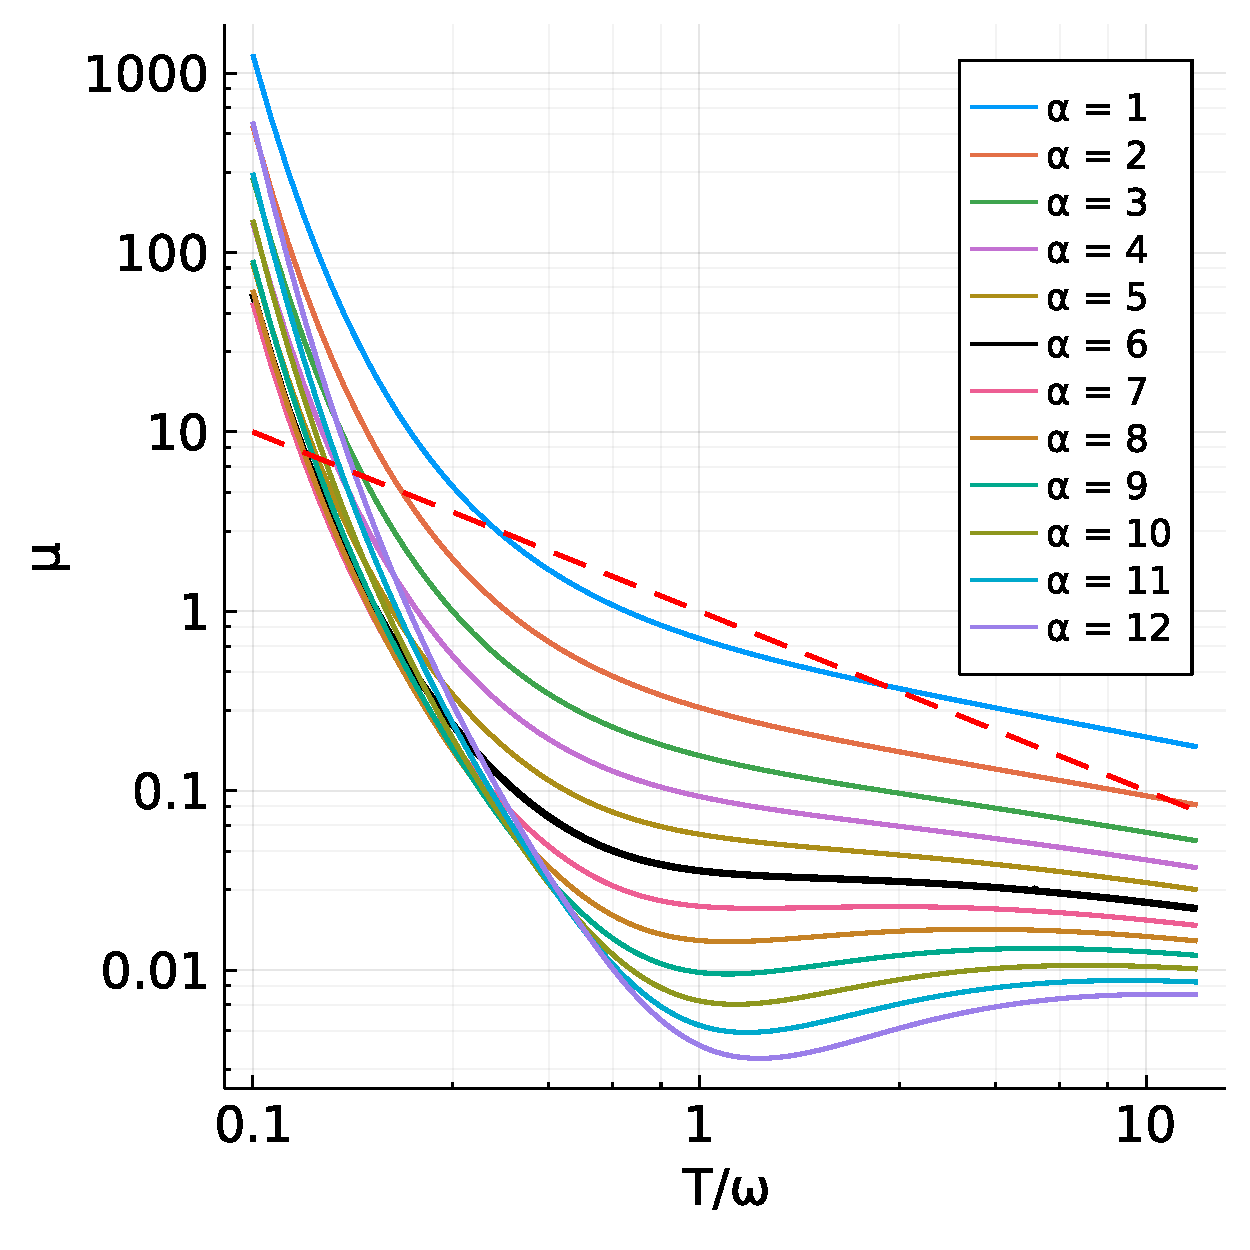
\includegraphics[width=.49\textwidth]{figures/moblility_temp_alpha.pdf}
    \includegraphics[width=.49\textwidth]{figures/medium (1).png}
    
    \caption{Temperature dependence of the polaron mobility. The Mott-Ioffe-Regel (MIR) threshold is given by the red dotted lines. Left: Mobility obtained from the thermal FHIP theory with $v$ and $w$ variational parameters calculated for each temperature, for Fr\"ohlich alphas ranging from $\alpha = 1$ to  $12$. The temperature is given in units of the phonon frequency $\omega$. Right: Mobility obtained by~\cite{mishchenko_polaron_2019} using the diagrammatic Monte Carlo method for $\alpha = 6$. The temperature is in units of the phonon frequency $\Omega$.}
    \label{fig:mishchenko2}
\end{figure}

Mishchenko et al.~\cite{mishchenko_polaron_2019} use the diagrammatic Monte Carlo (DiagMC) method to study the mobility of a Fr\"ohlich polaron in the ``Beyond Quasiparticle'' regime. In this regime, the inelastic scattering rate exceeds the thermal energy of quasiparticles. This can be restated as the regime where the mean free path of the particle exceeds its de Broglie wavelength. This form coincides with the Mott-Ioffe-Regel (MIR) criterion, which is where the motion of quasiparticles is ill-defined. 

In Figure~\ref{fig:mishchenko2} are comparisons between the temperature dependence of the polaron mobility evaluated using the~\cite{feynman_mobility_1962} method (right) compared to the~\cite{mishchenko_polaron_2019} DiagMC method (left). The key features of the DiagMC plot (right) are the non-monotonic behaviour of the mobility and the evaluation of the mobility near and below the MIR threshold (given by the red dotted line). These two features are also seen in FHIP mobility. The main difference between the two results is that, whilst the mobility minimum arises from the DiagMC method at $\alpha = 6$, the minimum arises from the FHIP method at $\alpha \geq 7$ and is less prominent. 
\begin{figure}[t]
    \centering
    \includegraphics[width=.49\textwidth]{figures/Mischenko_comparison.pdf}
    \includegraphics[width=.49\textwidth]{figures/medium.png}
    
    \caption{Polaron mobility for $\alpha = 6$. Left: Mobility obtained from the thermal FHIP theory with $v$ and $w$ variational parameters calculated for each temperature. The electric field frequency and temperature are given in units of the phonon frequency $\omega$. Right: Mobility obtained by~\cite{mishchenko_polaron_2019} using the diagrammatic Monte Carlo method. The electric field frequency and temperature are in units of the phonon frequency $\Omega$.}
    \label{fig:mishchenko}
\end{figure}
The mobility evaluated below the MIR threshold is stated in~\cite{mishchenko_polaron_2019} to be ``beyond the quasiparticle'' regime. However, the model from~\cite{feynman_mobility_1962} can also reliably evaluate the mobility in this regime despite being a quasiparticle model of two fictitious masses coupled by a spring-like potential. Additionally, the FHIP can reproduce the mobility minimum, too. \cite{mishchenko_polaron_2019} suggest that the minimum emerges from the competition between the decreasing number of thermal excitations (which dominates at $T << \omega$) and a strong mass renormalisation (which is prominent for $T > \omega$). 

Figure~\ref{fig:mishchenko} compares the polaron mobility evaluated for a Fr\"ohlich alpha $\alpha = 6$. The left figure shows the polaron mobility obtained from the thermal Feynman polaron theory (evaluated with (Eq. \ref{eqn:FHIP_mobility}) for the dc polaron mobility). The right figure shows the polaron mobility obtained from~\cite{mishchenko_polaron_2019}'s DiagMC method. The position of the peaks between the two methods align for each temperature ($0.125, 0.25, 0.5, 1, 2, 4\  \&\ 8\ K/\omega$, where $\omega$ is the single phonon mode frequency). The main difference between the two methods is that the peaks evaluated from the Feynman polaron method are taller and sharper, whereas the peaks evaluated from~\cite{mishchenko_polaron_2019}'s DiagMC method are broader and shallower. 

The difference in peak widths between the two methods is likely due to the two-mass spring model approximation made in the Feynman method within the trial action in Eq. (\ref{eqn:thermal_trial_action}). This fixes the dynamical behaviour of Feynman's model \emph{a priori} since it only contains two harmonic degrees of freedom. The translation invariance of the Fr\"ohlich Hamiltonian then fixes one eigenmode at zero frequency. The frequency of the other mode and the relative spectral weight of the peaks are then the free parameters. This spectrum differs greatly from the true spectrum of the polaron and means that the FHIP polaron mobility may only contain a very crude approximation of the true dissipation of the polaron. The dynamical properties of the FHIP approximation are investigated more by~\cite{sels_dynamic_2016}.

\subsection{Multiple Phonon Mode Mobility}
\label{subsec:3-1-3}

To generalise the frequency-dependent mobility in Eq.~(\ref{eqn:freq_dep_mobility}), I follow the same procedure as FHIP but use our generalised polaron action $S$ in Eq. (\ref{eqn:multiaction}) and trial action $S_0$ in Eq. (\ref{eqn:multi_trial_action}). The result is a memory function akin to Eq. (\ref{eqn:fhip_chi}) that is inclusive of multiple ($m$) phonon branches $j$ and multiple ($2n$) variational parameters $v_{p}$ and $w_{p}$,
\begin{equation} \label{eqn:multi_memory}
    \begin{gathered}
        \chi(\Omega) = \sum_{j=1}^m \frac{2\alpha_j}{3\sqrt{\pi}} \int_0^{\infty} dt\ \left[1 - e^{i\Omega t / \omega_j}\right] \textrm{Im} S_j(t)
    \end{gathered}
\end{equation}
where
\begin{equation}
    S_j(\Omega) = \frac{\cos \left(t - i\beta_j/2\right)}{\sinh (\beta_j/2)} [D_j(t)]^{-3/2}
\end{equation}
where $D(t)$ is just $D_j(it)$ from Eq. (\ref{eqn:multi_D}) rotated back to real-time to give a generalised version of $D(u)$ in Eq. (\ref{eqn:D_FHIP}) from FHIP,
\begin{equation}
    \begin{gathered}
        D_j(t) \equiv D_j(it) = 2\sum_{p=1}^n \frac{h_p}{v_{p}^3} \frac{\sin(v_{p} t/2) \sin(v_{p}[t-i\beta_j]/2)}{\sinh(v_{p}\beta_j/2)} \\
        -i \left(1-\sum_{p=1}^n\frac{h_{p}}{v_{p}^2}\right) t \left(1 - \frac{t}{i\beta_j}\right).
    \end{gathered}
\end{equation}
The new multiple-phonon frequency-dependent mobility $\mu(\Omega)$ is then obtained from the real and imaginary parts of the generalised $\chi$ using Eq.~(\ref{eqn:freq_dep_mobility}). The frequency-dependent mobility $\mu(\Omega)$ is obtained from the impedance using
\begin{equation}\label{eqn:freq_dep_mobility}
\begin{gathered}
    \mu(\Omega)^{-1} = \frac{m_b}{e} \sum_j^m \omega_j \textrm{Re}\left\{z_j(\Omega)\right\}
    = \frac{m_b}{e} \sum_j^m \omega_j \frac{\Omega^4 - 2\ \Omega^2\  \textrm{Re}\chi_j(\Omega) + |\chi_j(\Omega)|^2}{\Omega\ \textrm{Im}\chi_j(\Omega)}
    \end{gathered}
\end{equation}
where $\chi_j(\Omega)$ is just the $j$th component of $\chi(\Omega)$. The limit that the frequency $\Omega \rightarrow 0$ gives the FHIP dc-mobility extended to multiple phonon modes,
\begin{equation}
    \mu^{-1}_{dc} = \frac{m_b}{e}\lim_{\Omega \rightarrow 0} \sum_{j=1}^m \omega_j \frac{\textrm{Im}\chi_j(\Omega)}{\Omega}
\end{equation}
since $\textrm{Re}\chi(\Omega = 0) = 0$.

\subsubsection{Numerical integration of the memory function $\chi(\Omega)$}

In FHIP~\cite{feynman_mobility_1962}, and DSG~\cite{devreese_optical_1972}, they first convert the integral in the complex memory function $\chi(\Omega)$ (Eq. (\ref{eqn:fhip_chi})) to a contour integral (Eq. (\ref{eqn:contour_imX})) (I provide more details in Appendix A). The contour integral is then evaluated by expanding it as an infinite power series in terms of $K$ and Bessel functions with an imaginary argument. 

% I investigated three methods for evaluating the real and imaginary components of the complex memory function: $(1)$ direct Gauss-Kronrod quadrature integration of the memory function in Eqs. (\ref{eqn:fhip_chi}) and (\ref{eqn:multi_memory}); $(2)$ Gauss-Kronrod integration of the contour integrals (Eq. (\ref{eqn:contour_imX}) and a corresponding contour integral of the multiple phonon memory function (\ref{eqn:multi_memory})); and $(3)$ using the power series expansions of Bessel functions. I found that the contour integrals were doubly oscillatory and became unstable towards high frequencies ($\gtrapprox 30$ multiples of the phonon mode frequency $\omega_{LO}$). The power series expansions required arbitrary-precision floating-point numbers to avoid diverging at low temperatures or high frequencies. Therefore, method $(1)$, direct Gauss-Kronrod quadrature integration of the original integrals, was the most numerically stable and my chosen method for evaluating the complex memory functions.

\subsection{Multiple Fictitious Particle Mobility}

To generalise the frequency-dependent mobility in Eqn. (\ref{eqn:mobility}), we follow the same procedure as FHIP but use our generalised polaron trial action $S_0$ in Eqn. (\ref{eqn:multi_trial_action}). The result is a memory function akin to FHIP's $\chi$ (Eqn. (35) in \cite{Feynman1962}), but includes multiple ($2n$) variational parameters $v_{p}$ and $w_{p}$,
\begin{equation}\label{eqn:multichi}
    \begin{gathered}
        \chi(\Omega) = \frac{\alpha \omega_0^{2}}{3\sqrt{\pi}} \int_0^{\infty} dt\ \left[1 - e^{i\Omega t}\right] \textrm{Im} S(t)
    \end{gathered} .
\end{equation}
Here, 
\begin{equation}
    S(t) = D_{\omega_0}(t) [G(t)]^{-3/2} ,
\end{equation}
where $G(t)$ is $G(\tau = i t)$ from Eqn.~(\ref{eqn:multi_D}) rotated back to real-time to give a generalised version of $D(u)$ in Eqn.~(35c) in FHIP,
\begin{equation}
    \begin{gathered}
         G(t) = i t  \left(1 - \frac{i t}{\hbar\beta}\right) + \sum_{p=1}^n \frac{h_p}{v_p^3} \left(D_{v_p}(0) - D_{v_p}(\tau) - iv_p t\left(1 - \frac{it}{\hbar\beta} \right) \right).
    \end{gathered}
\end{equation}
The new frequency-dependent mobility $\mu(\Omega)$ is then obtained from the real and imaginary parts of the generalised $\chi(\Omega)$ using Eqn. (\ref{eqn:mobility}).

\subsubsection{The Effect on Dynamics}

\begin{figure}[!tbp]
    \centering
  \begin{subfigure}[b]{0.49\textwidth}
    \centering
    \includegraphics[width=\textwidth]{figures/cond_freq_bad.png}
  \end{subfigure}
  \hfill
  \begin{subfigure}[b]{0.49\textwidth}
    \centering
    \includegraphics[width=\textwidth]{figures/cond_alpha.png}
  \end{subfigure}
  \caption{Real component of the complex conductivity $\Re \sigma(\Omega)$ for the Fr\"ohlich model for increasing number $N$ of fictitious particles in the trial model. \textbf{Left:} The frequency-dependence of the real conductivity at $\alpha = 6$ and $\beta\omega_0=12.375$. Here I are in the regime for the maximum potential improvement on the trial model with the additional of fictitious particles. Despite minor improvements on the free energy approximation, the corresponding prediction for the real conductivity changes drastically due to the sensitivity of analytic continuation of the trial model. \textbf{Right:} Dependence of the ground-state ($T = 0$ K) real conductivity with the dimensionless electron-phonon coupling $\alpha$. The real conductivity converges quickly to its optimal solution as soon as $N=3$ with the maximal improvement occurring around $\alpha = 6$.}
  \label{fig:multidyn}
\end{figure}
Given that the multiple fictitious particle trial model rapidly converges to the optimal bound on the polaron-free energy, it is constructive to investigate how the dynamics of the trial system are altered. In Figs. (\ref{fig:multidyn}) the left figure shows the frequency-dependent conductivity at $\alpha = 6$ and thermodynamic temperature $\beta = 12.375 \omega_0$ for a number of fictitious particles coupled to the electron $N = 1, 2, 3$ and $4$. This is a regime where, from our previous observations, we expect to be close to the maximum potential improvement to the trial model by adding more fictitious particles. All four trial models agree at low frequencies below the phonon frequency. However, upon reaching the phonon frequency and beyond, we see that each trial model produces a conductivity with different oscillation periods and amplitudes. The frequency of this oscillation is smallest for the $N=1$ trial model and increases with each additional particle. Meanwhile, the amplitude of the oscillation decreases with more particles. The right figure shows the coupling dependence of the conductivity at zero temperature for $N=1, 2,3$ and $4$. This figure shows that the maximum improvement in the zero-temperature conductivity is around $\alpha = 6$ with little discernible difference between $N=3$ and $4$. Despite the apparent convergence of the conductivity for $N=3$ and $N=4$, the frequency dependence shows a significant difference, suggesting that far more fictitious particles may be required to reach a truly converged optimal solution in the frequency response of the trial system.

\subsection{The Holstein Model}

We can specialise in the Holstein model by substituting,
\begin{subequations}
    \begin{equation}
        \abs{V_{\vb{q}}}^2 = g_H^2(n) / N ,
    \end{equation}
    \begin{equation}
        \omega_{\vb{q}} = \omega_0 ,
    \end{equation}
    \begin{equation}
        \Lambda = 2\sqrt{\pi} \left(V \Gamma\left(\frac{n}{2} + 1\right)\right)^{1/n} \equiv \Lambda_n .
    \end{equation}
\end{subequations}
The $q$-space integral is evaluated,
\begin{equation}
    \begin{aligned}
    I^{(H)}(n) &= \frac{g^2_H(n) V \abs{S^{n-1}}}{N (2\pi)^n} D_{\omega_0}(t) \int_0^{\Lambda_n} dq\ q^{n+1} e^{-q^2 r_p^2 G(t)} , \\
    &= \frac{g^2_H(n) \abs{S^{n-1}}}{2 (2\pi)^n r_p^{n+2}} \frac{V}{N} 
    \frac{D_{\omega_0}(t)}{G(t)^{\frac{n}{2}+1}} \left[ \Gamma\left(\frac{n}{2} +1\right) - \Gamma\left(\frac{n}{2}+1, r_p^2 \Lambda_n^2 G(t) \right) \right] , \\
    &= \frac{1}{2 r_p^2} \frac{V}{N} \frac{n g_H^2(n)}{(2 r_p \sqrt{\pi})^n} \frac{D_{\omega_0}(t)}{G(t)^{\frac{n}{2}+1}} \left[ 1 - \frac{\Gamma\left(\frac{n}{2} + 1, r_p^2 \Lambda_n^2 G(t) \right)}{\Gamma\left(\frac{n}{2} + 1\right)} \right] .
    \end{aligned}
\end{equation}
The memory function for the Holstein model is then:
\begin{equation}
    \Sigma^{(H)}(\Omega) = \frac{\rho}{m_b\hbar\Omega \gamma r_p^{n+2}} \frac{4 n \alpha^{(H)}}{(2 \sqrt{\pi})^n} \int_0^\infty dt\ \left(1 - e^{i \Omega t}\right) \frac{D_{\omega_0}(t)}{G(t)^{\frac{n}{2}+1}} \left[ 1 - \frac{\Gamma\left(\frac{n}{2} + 1, r_p^2 \Lambda_n^2 G(t) \right)}{\Gamma\left(\frac{n}{2} + 1\right)} \right],
\end{equation}
and where $\rho = V / N$ is the particle density and $\gamma = \hbar\omega_0 / J$ is the adiabaticity. The inverse Holstein DC mobility is then,
\begin{equation}
    \mu_{dc}^{-1} = \frac{\rho e^2}{m_b\hbar \gamma r_p^{n+2}} \frac{4 n \alpha^{(H)}}{(2 \sqrt{\pi})^n} \int_0^\infty dt\ t \frac{D_{\omega_0}(t)}{G(t)^{\frac{n}{2}+1}} \left[ 1 - \frac{\Gamma\left(\frac{n}{2} + 1, r_p^2 \Lambda_n^2 G(t) \right)}{\Gamma\left(\frac{n}{2} + 1\right)} \right].
\end{equation}

\subsubsection{Polaron Mobility}

\begin{figure}[!tbp]
    \includegraphics[width=.49\textwidth]{figures/mobility_temp_25_083.png}
    \includegraphics[width=.49\textwidth]{figures/mobility_temp_4_133.png}
    \includegraphics[width=.49\textwidth]{figures/mobility_temp_6_2.png}
    \includegraphics[width=.49\textwidth]{figures/mobility_temp_8_267.png}
    \includegraphics[width=.49\textwidth]{figures/mobility_temp_10_333.png}
    \includegraphics[width=.49\textwidth]{figures/mobility_temp_12_4.png}
    \caption{Temperature dependence ($T$, in units of phonon frequency $\omega_0$) of the polaron DC mobility $\mu$ for the Fr\"ohlich model in 2D (solid blue) and 3D (dashed orange), and for the Holstein model in 1D (dot-dashed green), 2D (dot-dot-dashed pink) and 3D (solid gold), for values of the Fr\"ohlich electron-phonon coupling $\alpha = 2.5, 4, 6, 8, 10, 12$ and $1/3$ of these values for the Holstein electron-phonon coupling.}
    \label{fig:mobility_temp}
\end{figure}
In Figs. (\ref{fig:mobility_temp}) we have the temperature dependence of the polaron mobility for the Holstein polaron with varying electron-phonon coupling. At weaker coupling, mobility shows the typical exponentially decreasing band-like transport at temperatures below the phonon energy level. Above the phonon energy, the temperature dependence transitions to a power-law relationship $T^{-x}$ where $x$ is some number that is typically used to determine the dominant scattering mechanism within a material. For example, this index is typically $x = 3/2$ for acoustic phonons. 

Again, as we saw previously, 2D Holstein and 3D Fr\"ohlich appear to be most alike. As the electron-phonon coupling increases, we begin to see the onset of the ski-slope feature where the mobility takes on a local minimum at the phonon energy $T = \omega_0$ before increasing to a local maximum at the polaron quasiparticle frequency $v$ and then transitioning back into a power-law relationship at higher temperatures. Each of the different dimensions of both polaron models seems to have a different dependence on the strength of the electron-phonon coupling when it comes to mobility. For the Fr\"ohlich polaron, the ski-slope appears sooner for the 2D model than the 3D model. For the Holstein polaron, the opposite trend seems to be true, with the higher dimension model exhibiting the ski-slope. The 2D Fr\"ohlich polaron also seems to manifest a low-temperature maximum at larger electron-phonon couplings, which transitions in a linear decrease to some finite value in mobility as the temperature goes to zero.

At high temperatures, the Fr\"ohlich polaron mobility follows the temperature power-law $\mu^{(H)} \sim T^{-1/2}$, which is consistent with mobility derived from the electron scattering with optical phonons. However, the Holstein polaron mobility becomes constant at high temperatures, independent of temperature. This may be attributed to the phonon-induced electron hopping between lattice sites along which the electron motion is coherent in the direction of that particular energy band. Likewise, at low temperatures, the mobility increases abruptly below the Debye temperature due to the increasing contribution of the electron transfer without phonon participation.

\section{Frequency-Dependent Optical Conductivity}
\label{sec:5-2}

\subsection{Holstein Model}
\label{subsec:5-2-1}

In this section, we look at how the Holstein model varies with an external, perturbing, and varying electric field frequency. Specifically, the polaron memory function, which we compare to the Fr\"ohlich polaron results of FHIP~\cite{feynman_mobility_1962}, and the optical conductivity, which we compare to the Fr\"ohlich polaron results of DSG~\cite{devreese_optical_1972}. For the memory function we look at frequencies $\Omega / \omega_0$ from $0$ to $28$ and $\alpha^{(F)} = 3, 5, 7$ or $\alpha^{(H)} = 1, 1.67, 2.33$. For the optical conductivity we look at frequencies $\Omega / \omega_0$ from $0$ to $11$ for $\alpha^{(F)} = 1, 3, 5, 6$ or $\alpha^{(H)} = 0.33, 1, 1.67, 2$ and frequencies $\Omega / \omega_0$ from $0$ to $22$ for $\alpha^{(F)} = 7$ or $\alpha^{(H)} = 2.33$. 

\subsubsection{Polaron Memory Function}

\begin{figure}
\centering
  \begin{subfigure}[b]{0.49\textwidth}
    \includegraphics[width=\textwidth]{figures/im_mem_freq_3_1.png}
  \end{subfigure}
  \hfill
  \begin{subfigure}[b]{0.49\textwidth}
    \includegraphics[width=\textwidth]{figures/im_mem_freq_5_167.png}
  \end{subfigure}
  \begin{subfigure}[b]{0.49\textwidth}
    \centering
    \includegraphics[width=\textwidth]{figures/im_mem_freq_7_233.png}
  \end{subfigure}
  \caption{Frequency dependence ($\Omega$, in units of the phonon frequency $\omega_0$) of the polaron memory function $\chi(\Omega)$ for the Fr\"ohlich model in 3D (solid blue), and the Holstein model in 1D (dashed orange), 2D (dot-dashed green) and 3D (solid gold), for values of the Fr\"ohlich electron-phonon coupling $\alpha = 1, 3, 5,6, 7$ and $1/3$ of these values for the Holstein electron-phonon coupling. Here, I only consider the imaginary component to reduce graph clutter, but the real component was also evaluated.} 
  \label{fig:im_mem_freq}
\end{figure}
In Figs. (\ref{fig:im_mem_freq}) is the frequency-dependent imaginary component of the memory function for the Holstein and Fr\"ohlich polarons for a range of electron-phonon coupling strengths. I chose these specific alpha values $\alpha^{(F)} = 3, 5, 7$ for direct comparison to figures (1-3) in FHIP~\cite{feynman_mobility_1962}. Note that here we use Devreese and Peeter's definition of the memory function $\Sigma(\Omega)$~\cite{peeters_theory_1984}, which is related to the FHIP memory function $\chi(\Omega)$ by the expression $\Sigma(\Omega) = \chi(\Omega) / \Omega$. I have excluded the 2D Fr\"ohlich result as even at `weak' coupling, it behaves like the 3D Fr\"ohlich result at strong coupling and is difficult to compare with.

The first most noticeable observation is that the 1D Holstein memory function seems to most closely relate to the 3D Fr\"ohlich memory function. This also is not surprising because the $q$-space integral in the memory function $\Sigma(\Omega)$ is the same for the 3D Fr\"ohlich and 1D Holstein polarons. Additionally, the imaginary component of the memory function is zero for frequencies below the phonon frequency, and the first peak corresponds to one phonon excitation.

As the electron-phonon coupling strength increases, more oscillations manifest at multiples of the polaron quasiparticle frequency $\Omega_{\text{peaks}} = 1 + n v, n \in \mathbf{N}$ which correspond to two- three- four etc phonon excitations. These peaks are significantly stronger in the Holstein polaron. 

The 2D and 3D Holstein memory functions take very different forms from what is seen for the 1D Holstein and 3D Fr\"ohlich polarons. At lower coupling, there seems to be more of a background lattice response that obscures the underlying phonon excitations until the small polaron state is formed at $\alpha^{(H)} > 2$.

\subsubsection{Polaron Optical Conductivity}

\begin{figure}[!tbp]
    \centering
    \includegraphics[width=.49\textwidth]{figures/re_con_freq_1_033.png}
    \includegraphics[width=.49\textwidth]{figures/re_con_freq_3_1.png}
    \includegraphics[width=.49\textwidth]{figures/re_con_freq_5_167.png}
    \includegraphics[width=.49\textwidth]{figures/re_con_freq_6_2.png}
    \includegraphics[width=.49\textwidth]{figures/re_con_freq_7_233.png}
    \caption{Frequency dependence ($\Omega$, in units of the phonon frequency $\omega_0$) of the polaron complex conductivity $\sigma(\Omega)$ for the Fr\"ohlich model in 2D (solid blue) and 3D (dashed orange), and for the Holstein model in 1D (dotted green), 2D (dot-dashed pink) and 3D (d pink), for values of the Fr\"ohlich electron-phonon coupling $\alpha = 3, 5, 7$ and $1/3$ of these values for the Holstein electron-phonon coupling. Here, I only consider the imaginary component to reduce graph clutter, but the real component was also evaluated.}
    \label{fig:re_con_freq}
\end{figure}
In Figs. (\ref{fig:re_con_freq}) is the frequency-dependent real component of the complex conductivity (otherwise known as the optical conductivity) for the Holstein and Fr\"ohlich polarons for a range of electron-phonon coupling strengths. I chose these specific alpha values $\alpha^{(F)} = 1, 3, 5, 6, 7$ for direct comparison to Figs.~(1-5) in DSG~\cite{devreese_optical_1972}.

Starting at weak coupling $\alpha^{(F)} = 1, \alpha^{(H)} = 0.33$, both models in all the presented spatial dimensions show the same form of a one-phonon excitation peak that decays away at higher frequencies. At intermediate coupling, we begin to see more structure. Firstly, the 2D Fr\"ohlich polaron shows many peaks and side bands that are only made apparent in the 3D Fr\"ohlich polaron at strong coupling. At $\alpha^{(F)} = 3$, we already see a very intense relaxed excited state (RES) transition occurs for Fr\"ohlich 2D followed by a prominent Frank-Condon (FC) excitation peak. Conversely, the other Fr\"ohlich 3D and Holstein 1D, 2D and 3D only exhibit the initial one-phonon peak with no apparent RES transitions or FC peaks. At $\alpha^{(F)} = 5, \alpha^{(H)} = 1.67$, the features of the 2D Fr\"ohlich polaron are pushed to very high frequencies far beyond the other polarons. However, the 3D Fr\"ohlich polaron only just begins to develop a RES transition peak around $\Omega = v$ with the shoulder on the low-frequency side representing the original one-phonon peak and the additional peak on the high-frequency side representing a FC band. The Holstein polaron still only possesses the one-phonon peak for 1D, 2D and 3D. This pattern continues until we exceed $\alpha^{(H)} = 2$. Unlike the Fr\"ohlich polaron, which developed RES and FC peaks before its polaron transition, the Holstein polaron does not develop these features until the coupling increases beyond $\alpha^{(H)} = 2$ where a small polaron state is formed, at which point the onset of strong RES and FC states is far more rapid than for the Fr\"ohlich polaron. 

\section{The Optimal Self-Consistent Response Function}
\label{sec:chap-fifth-third}

\subsection{Statics = Dynamics}

The function $\Sigma(\Omega)$, which gives the lowest energy in the variational principal at zero temperature, satisfies the integral equation,
\begin{equation}
    \Sigma(\Omega) = \frac{2}{n} \sum_{\vb{q}} \abs{V_{\vb{q}}}^2 q^2 \int^\infty_0 d\tau \left( 1 - \cos(\Omega \tau) \right)  e^{-\omega_{\vb{q}} \tau} e^{-q^2 r_p^2 [G(0) - G(\tau)]}, 
\end{equation}
where,
\begin{equation}
    G(\tau) = \int_{-\infty}^\infty \frac{d\omega}{2\pi} \frac{ e^{i \omega \tau} }{m \omega^2 - \Sigma(\omega)} .
\end{equation}
The polaron Green's function $G(\tau)$ that minimises the polaron free energy at arbitrary temperature without applied electric and magnetic fields also produces the optimal impedance function $z(\Omega)$. 

Generalising the variational equations to a general polaron system, we obtain,
\begin{equation}
    F \leq \frac{n}{\beta} \sum_{l=1}^\infty \ln \left( \frac{Z(\omega_l)}{m \omega_l^2} \right) - \frac{n}{\beta} \sum_{l=1}^\infty \frac{1 - m \omega^2_l}{Z(\omega_l)} - \int_0^{\frac{\hbar\beta}{2}} d\tau \sum_{\vb{q}, j} \abs{V_{\vb{q}, j}}^2 D_{\vb{q}, j}(\tau) e^{-q^2 r_p^2 \left[G(0) - G(\tau)\right]},
\end{equation}
where,
\begin{equation}
    \Sigma(\tau) = \frac{2}{\beta} \sum_{l = 1}^\infty \frac{1 - \cos\left(\omega_l \tau \right)}{Z(\omega_l)},
\end{equation}
and,
\begin{equation}
    Z(\omega_l) = m \omega_l^2 + 4 \int_{-\infty}^\infty d\Omega \frac{P}{\Omega} \frac{G(\Omega) \omega^2_l}{\Omega^2 + \omega_l^2},
\end{equation}
and $\omega_l \equiv 2\pi l / \beta$, $l \in \mathbf{N}$.